
\documentclass[times,singlecolumn]{article}
\usepackage[margin=1in]{geometry}
\usepackage{amsmath}
\usepackage{amsfonts}
\usepackage{graphicx}
\usepackage{xcolor}
\usepackage{ulem}
\usepackage{hyperref}
\input{sym}

\newcommand{\ubfu}{\underline{\bfu}}
\newcommand{\ubfx}{\underline{\bfx}}

\newtheorem{prob}{Problem}


\title{ECE 417/598: Rotation from P matrix}
\author{Instructor: Vikas Dhiman}
\DeclareMathOperator{\diag}{diag}
\begin{document}
\maketitle
\begin{tabular}{p{0.5\linewidth}p{0.5\linewidth}}
  (1) Student name:& Student email: \\
\end{tabular}

\begin{prob}
  Find the 3D position of the pothole give that the right camera $r$  is moved
  along X-axis by $b=1m$ with respect to the left camera $L$. 
\end{prob}

\includegraphics[width=\linewidth]{media/image-road-triangulation-ray-ray.pdf}

\newpage
\begin{enumerate}
\item Find the equation of ray corresponding to the pothole in the left image.
  In other words, write the equation of the ray corresponding to the point
  $\ubfu_L$, in camera frame $L$.
  \vspace{10em}

\item Find the rotation matrix ${}^rR_L$ and translation vector ${}^r\bft_L$, so
  that they transform any point in the coordinate frame $L$ to a point in the
  coordinate frame $r$. ($\bfX_r = {}^rR_L \bfX_L + {}^r\bft_L$).
  \vspace{10em}

\item Transform the equation of ray from coordinate frame $L$ to coordinate
  frame $r$.
  \label{enit:left-ray}
  \vspace{10em}

\item Find the equation of ray corresponding to the pothole in the right image.
  In other words, write the equation of the ray corresponding to the point
  $\ubfu_r$, in camera frame $r$.
  \label{enit:right-ray}
  \vspace{10em}

\item Find the intersection of rays (lines) \ref{enit:right-ray} and \ref{enit:left-ray}.
  \vspace{10em}
\end{enumerate}

\newpage
\begin{prob}
  When the depth corresponding to the point $\bfx$ is unknown, the possible
  pixels ($\bfx'$) on the right image that can correspond to  the point form a
  line. What is the equation of that line?
  \\
  \includegraphics[width=0.5\linewidth]{media/epipolar-line.png}
\end{prob}

\begin{enumerate}
\item Find the equation of ray corresponding to the pothole in the left image.
  In other words, write the equation of the ray corresponding to the point
  $\bfx$, in the first camera frame.
  \vspace{8em}

\item Assume the rotation matrix $R$ and translation vector $\bft$, so
  that they transform any point in the left coordinate frame to a point in the
  right coordinate frame. ($\bfX' = R \bfX+ \bft$). Transform the equation of
  ray from the left coordinate frame to the right coordinate frame.
  \vspace{8em}

\item Project any 3D point on the  right camera, call it $\bfx'$.
  \vspace{8em}

\item Find the point $\bfe'$ on the right camera.
  \vspace{8em}

\item Find a line $\bfl'$ that passes through both $\bfx'$ and $\bfe'$.
  \vspace{8em}

\end{enumerate}

\newcommand{\ubfX}{\underline{\bfX}}
\newpage
\begin{prob}
  Given a set of $n \ge 6$ points $\ubfX_i \in \bbP^3$ for all $i \in \{1,
  \dots, n\}$ in 3D projective space, and a set
  of corresponding points $\ubfu_i \in \bbP^2$ in an image, find the 3D to 2D projective
  $P \in \bbR^{3 \times 4}$ matrix
  that converts $\bfX_i$ to $\ubfu_i  =  \lambda_i P\ubfX_i$. In other words,
  convert $\ubfu_i \times P\ubfX_i = 0$ into a familiar form $A\bfy = \bfb$ or
  $A\bfy = \mathbf{0}$ so that we can solve for $P$. For notation purposes, you can
  denote $\ubfu_i = [x_i, y_i, w_i]^\top$ and $P = \begin{bmatrix}
    \bfp_1^\top \\ \bfp_2^\top \\ \bfp_3^\top \end{bmatrix}$ where $\bfp_1,
  \bfp_2, \bfp_3 \in \bbR^4$ are the rows of $P$ represented as 4-D column vectors.
  (Practical motivation:
    We did camera calibration in lab using a single checker board. It is much
    easier to compute camera calibration using two mutually perpendicular checker
    boards so that all points do not lie on a single plane (hence linearly
    independent). One can make a coordinate system attached to the double checker
    and compute the 3D coordinates of each corner point in that system. Let
    $\ubfX_i \in \bbP^3$ be such points in 3D on the checker-board. Let $\ubfu_i
    \in \bbP^2$ be a point detected in the image so that we have one-to-one
    correspondence between $\ubfX_i$ and $\ubfu_i$. Finding the projection matrix
    $P \in \bbR^{3 \times 4}$ then reduces to the above problem. We will cover
    the breakdown of $P$ matrix into $P = K[R, t]$ in class.
  ) \\
  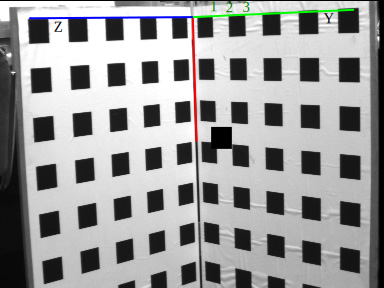
\includegraphics[width=0.5\linewidth]{media/camera-calibration-rig.png.pdf}
\end{prob}
\newpage
\paragraph*{Solution}
Watch lecture \url{https://drive.google.com/file/d/1cY02DTagpckbYl5gS0PYBu569vlZUNN6/view?usp=sharing}
\begin{enumerate}
\item Write cross product as a matrix operation
  \[ [\ubfu_i]_{\times}= \begin{bmatrix}
      0 & -w_i & y_i \\
      w_i & 0 & -x_i \\
      -y_i & x_i & 0
    \end{bmatrix}\]
  \item Write $P \ubfX_i$ in terms of row vectors.
    \[ P \ubfX_i = \begin{bmatrix}
        \bfp_1^\top
        \\
        \bfp_2^\top
        \\
        \bfp_3^\top
      \end{bmatrix}\ubfX_i =  \begin{bmatrix}
        \bfp_1^\top\ubfX_i
        \\
        \bfp_2^\top\ubfX_i
        \\
        \bfp_3^\top\ubfX_i
      \end{bmatrix}\]
    \item Note that all the three terms like $\bfp_1^\top \ubfX_i$ are scalars
      hence they are symmetric. Hence $\bfp_1^\top \ubfX_i = \ubfX_i^\top \bfp_1$ .
      \[ P \ubfX_i = \begin{bmatrix}
          \ubfX_i^\top\bfp_1
                 \\
          \ubfX_i^\top \bfp_2
                 \\
          \ubfX_i^\top\bfp_3
        \end{bmatrix}\]
    \item Substitute these values in the original equation $\ubfu_i \times
      P\ubfX_i = \mathbf{0}_{3\times 1}$.
      \[
        \begin{bmatrix}
          0 & -w_i & y_i \\
          w_i & 0 & -x_i \\
          -y_i & x_i & 0
        \end{bmatrix}
        \begin{bmatrix}
          \ubfX_i^\top\bfp_1
          \\
          \ubfX_i^\top \bfp_2
          \\
          \ubfX_i^\top\bfp_3
        \end{bmatrix} = \mathbf{0}_{3 \times 1}
        \]
      \item Matrix multiply
        \[
          \begin{bmatrix}
            0 -w_i \ubfX_i^\top\bfp_2 + y_i \ubfX_i^\top\bfp_3 \\
            w_i \ubfX_i^\top\bfp_1 + 0  -x_i \ubfX_i^\top\bfp_3 \\
            -y_i \ubfX_i^\top\bfp_1 + x_i \ubfX_i^\top\bfp_2 + 0
          \end{bmatrix} = \mathbf{0}_{3 \times 1}
          \]
        \item Write the unknowns as a single vector, and the knowns as a matrix
          multiplication with the unknowns
          \[
            \begin{bmatrix}
              \mathbf{0}^\top & -w_i \ubfX_i^\top & y_i \ubfX_i^\top \\
              w_i \ubfX_i^\top & \mathbf{0}^\top  & -x_i \ubfX_i^\top \\
              -y_i \ubfX_i^\top & x_i \ubfX_i^\top & \mathbf{0}^\top
              \end{bmatrix}_{3 \times 12}
              \begin{bmatrix}
                \bfp_1 \\
                \bfp_2 \\
                \bfp_3
                \end{bmatrix}_{12 \times 1}
                = \mathbf{0}_{3 \times 1}
            \]
     \item Pick only two of the equations as only two are linearly independent.
       \[
         \begin{bmatrix}
           \mathbf{0}^\top & -w_i \ubfX_i^\top & y_i \ubfX_i^\top \\
           w_i \ubfX_i^\top & \mathbf{0}^\top  & -x_i \ubfX_i^\top
         \end{bmatrix}_{2 \times 12}
         \begin{bmatrix}
           \bfp_1 \\
           \bfp_2 \\
           \bfp_3
         \end{bmatrix}_{12 \times 1}
         = \mathbf{0}_{2 \times 1}
       \]
     \item Collect all the equations from $n$ pairs of corresponding points
       $\ubfu_1, \dots, \ubfu_n$ and $\ubfX_1, \dots, \ubfX_n$.
       \[
         \begin{bmatrix}
           \mathbf{0}^\top & -w_1 \ubfX_1^\top & y_1 \ubfX_1^\top \\
           w_1 \ubfX_1^\top & \mathbf{0}^\top  & -x_1 \ubfX_1^\top \\
           \vdots & \vdots & \vdots\\
           \mathbf{0}^\top & -w_n \ubfX_n^\top & y_n \ubfX_n^\top \\
           w_n \ubfX_n^\top & \mathbf{0}^\top  & -x_n \ubfX_n^\top \\
         \end{bmatrix}_{2n \times 12}
         \begin{bmatrix}
           \bfp_1 \\
           \bfp_2 \\
           \bfp_3
         \end{bmatrix}_{12 \times 1}
         = \mathbf{0}_{2n \times 1}
       \]
   \item $P$ matrix has rank $\text{rank}(P) = 11$ because it has 12 elements
     and equivalence upto a scale factor. So the solution of the above equation
     can be computed from SVD by choosing the right singular vector corresponding
     to the smallest singular value.
     \[
      A = \begin{bmatrix}
        \mathbf{0}^\top & -w_1 \ubfX_1^\top & y_1 \ubfX_1^\top \\
        w_1 \ubfX_1^\top & \mathbf{0}^\top  & -x_1 \ubfX_1^\top \\
        \vdots & \vdots & \vdots\\
        \mathbf{0}^\top & -w_n \ubfX_n^\top & y_n \ubfX_n^\top \\
        w_n \ubfX_n^\top & \mathbf{0}^\top  & -x_n \ubfX_n^\top \\
       \end{bmatrix} = U\Sigma V^T
     \]
     Let $V = [\bfv_1, \dots, \bfv_n]$, then
     \[
       \begin{bmatrix}
         \bfp_1 \\
         \bfp_2 \\
         \bfp_3
         \end{bmatrix} = \bfv_n
       \]

       Now we can write the $P$ matrix as
       \[
         P = \begin{bmatrix}
           \bfp_1^\top \\
           \bfp_2^\top \\
           \bfp_3^\top
         \end{bmatrix}
         \]
\end{enumerate}

\begin{prob}
  Given to vectors $\bfa$ and $\bfb$ find a set of unit vectors that are
  mutually orthonormal and write $\bfa$, $\bfb$. in terms of those mutually orthonormal vectors.
\end{prob}

\newpage
\begin{prob}
  Repeat the process for 3 vectors, $\bfa$, $\bfb$ and $\bfc$.
\end{prob}

\newpage
\begin{prob}
  Repeat the process for $n$ vectors, $\bfa_1$, $\bfa_2$ and $\bfa_3$.
\end{prob}

\end{document}